%!TEX root = ../main.tex
% chktex-file 46
\chapter{Learning to Decompose Graphs}%
\label{sec:ltd}

In the last chapter we saw how existing \ac{gcr} approaches relate to \ac{lta}.
Despite their differences, all described \ac{lta} formulations have one thing in common:
Their decomposition functions $\psi$ all split a given graph $G$ into constituents spanned by \ac{bfs} subtrees of $G$ or simply into connected components of $G$.
The only exception to this is the \ac{lta} formulation of \acp{svm} that use fingerprint embeddings; there the constituents are all isomorphic to handpicked substructures.

Apart from the fingerprint embedding approach, which requires domain knowledge in order to pick meaningful substructure patterns, current \ac{gcr} approaches use constituents that are at-best \textit{localized} but not necessarily \textit{interpretable}.
The defining characteristic of \ac{lta} proposed in \cref{sec:ltag:definition}, \textit{localized explainability}, is therefore only partially satisfied by existing approaches.
This shortcoming of the existing \ac{lta} formulations for structured input data gives rise to a new problem:
\begin{defn}
	The \ac{ltd} problem is solved by finding a graph decomposition function $\psi: \mathcal{G}_{\mathcal{D}} \to \mathcal{P}(\mathcal{G}_{\mathcal{D}})$ which splits all graphs $G \in \mathcal{G}_{\mathcal{D}}$ from a given domain $\mathcal{D}$ into constituent subgraphs which are individually ``meaningful'' in the domain $\mathcal{D}$.
\end{defn}

As per our definition of \ac{lta} from \cref{sec:ltag:definition}, the quality of an \ac{lta} formulation is determined by its chosen solution for the \ac{ltd} problem.
Since a comprehensive analysis of this problem would be beyond the scope of this thesis, we focus on the relation between \ac{ltd} and \acp{gcnn}.
The goal of this chapter is to answer the following two questions:
\begin{enumerate}
	\item \textit{Can a stack of graph convolution layers learn a decomposition function dynamically instead of using a static subtree decomposition?}
	\item \textit{What could be the foundation for such an ``\acs{ltd}-convolution'' layer?}
\end{enumerate}

We provide an answer to the first question in \cref{sec:ltd:edge-filter} by showing how decomposition functions $\psi$ can be learned via so-called \textit{edge filters} as part of a convolutional \ac{gnn} architecture.
This establishes the connection between the \acs{ltd} problem and graph convolutions on a high level.
Then the second question is tackled in \cref{sec:ltd:kgnn-limits,sec:ltd:wl2gnn}.
There a novel graph convolution approach is proposed which could serve as a starting point for a convolution layer which solves the \ac{ltd} problem.

\section{Learning Constituents via Edge Filters}%
\label{sec:ltd:edge-filter}

As we saw in \cref{sec:ltag:formulation:gcnn:conv}, the constituents of neighborhood convolutions are spanned by \ac{bfs} trees of depth $T$, where $T$ is the number of convolutional layers.
From this perspective the problem of learning constituents corresponds to learning a pruning operator on the branches of \ac{bfs} trees.
Such a pruning operator filters the edges that are traversed in each \ac{bfs} step.
There are two general edge filtering strategies:
\begin{enumerate}[label={\textbf{\arabic*.}}]
	\item \textbf{Edge prefiltering:}
		Here the edge filtering and convolution operations are performed in independent steps:
		First the edges of a given graph are filtered, then the convolution layers are applied to the filtered graph.
		This so-called \textit{edge prefiltering} strategy is illustrated in \cref{fig:ltd:subtree-filtering}.
		The main advantage of prefiltering is that it allows arbitrary combinations of edge filtering and convolution approaches.
		The main disadvantage is however that the same edges are removed in all \ac{bfs} subtrees.
		This restricts the expressive power of the learned decomposition function as shown in \cref{fig:ltd:dynamic-subtree-filtering}.
	\item \textbf{Dynamic edge filtering:}
		By filtering edges as part of the convolution operation itself, more flexible decompositions can be obtained.
		In the \textit{dynamic edge filtering} strategy the edge filter is part of the convolution operation and decides which neighbors of a given root node should be aggregated.
		Using this strategy a decomposition such as that shown in \cref{fig:ltd:dynamic-subtree-filtering} is learnable.
\end{enumerate}
\begin{figure}[ht]
	\centering
	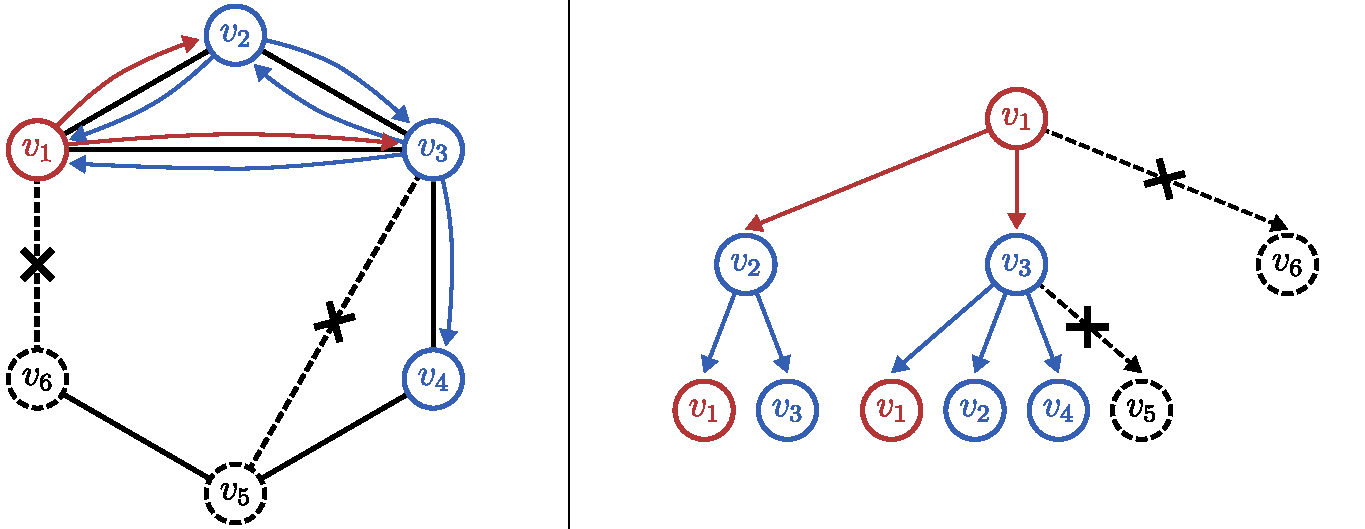
\includegraphics[width=0.8\linewidth]{gfx/ltd/subtree-filtering.pdf}
	\caption{Illustration of a pruned \ac{bfs} subtree when two edges are removed via prefiltering.}\label{fig:ltd:subtree-filtering}
\end{figure}
\begin{figure}[ht]
	\centering
	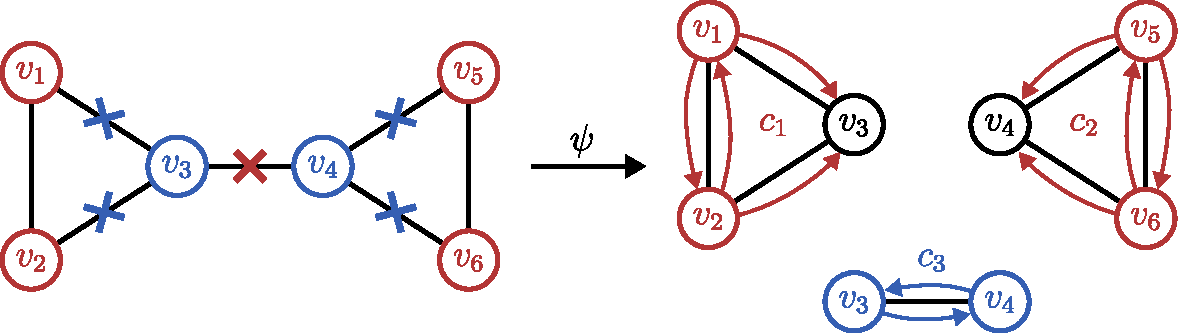
\includegraphics[width=0.75\linewidth]{gfx/ltd/dynamic-subtree-filtering.pdf}
	\caption[A graph decomposition obtained via dynamic edge filtering which cannot be modeled by edge prefiltering.]{
		A graph decomposition obtained via dynamic edge filtering which cannot be modeled by edge prefiltering.
		Depending on the \ac{bfs} root node $v_{\mathrm{root}}$ different edges are removed.
		For $v_{\mathrm{root}} \in \textcolor{t_blue}{\{ v_3, v_4 \}}$ the edges $\{ (v_3, v_1), (v_3, v_2), (v_4, v_5), (v_4, v_6) \}$ are filtered out while for $v_{\mathrm{root}} \in \textcolor{t_red}{\{ v_1, v_2, v_5, v_6 \}}$ the edge $(v_3, v_4)$ is removed. % chktex 25
	}\label{fig:ltd:dynamic-subtree-filtering}
\end{figure}
Irrespective of the chosen edge filtering strategy, the decision whether to remove a given edge $e_{ij} = (v_i, v_j)$ or not has to be made based on relevant information about $e_{ij}$ and its surroundings.
One way to encode the information about $e_{ij}$ is via an edge feature vector $z_{ij} \in \mathbb{R}^d$ that is fed into the edge filter.

We propose that those edge feature vectors can be obtained via a 2-\acs{wl} inspired graph convolution layer since 2-\acs{wl} colors naturally represent the structural roles of edges as described in \cref{sec:related:character:wl}.
We already saw a \ac{gcnn} architecture in \cref{sec:related:gcr:nn} which could potentially compute such 2-\acs{wl} inspired edge feature vectors, the $k$-\acs{gnn}~\cite{Morris2019}.
Its variant for $k = 2$ produces edge feature vectors that can be used as the input for an edge filter.
However, as we will see in the next section, there are significant limitations to the discriminative and computational power of 2-\acsp{gnn}.

\section{Limitations of the Existing 2-\acs*{gnn}}%
\label{sec:ltd:kgnn-limits}

The $k$-\acs{gnn} is a \ac{gcnn} inspired by the $k$-\ac{wl} algorithm, it convolves feature vectors of vertex $k$-multisets.
In this section we will compare its $k = 2$ variant with the 2-\ac{wl} algorithm.
The main difference between the two boils down to their notion of ``neighborhood''.
As already briefly mentioned in \cref{sec:related:gcr:nn}, 2-\acsp{gnn} define the neighbors of an edge $\textcolor{t_blue}{e_{ij}} = (v_i, v_j)$ to be the edges that are incident to either $v_i$ or $v_j$. % chktex 25
In 2-\acs{wl} on the other hand, the neighbors of $\textcolor{t_blue}{e_{ij}}$ are the edge pairs ${\left\{(\textcolor{t_red}{e_{il}}, \textcolor{t_darkgreen}{e_{lj}})\right\}}_{v_l \in \mathcal{V}_G}$, i.e.\ all possible paths of length two that start at $v_i$ and end at $v_j$. % chktex 21 chktex 25
This difference becomes clear when comparing the definition of convolution in 2-\acsp{gnn} with that of color refinement in 2-\acs{wl} (see \cfullref[ on ]{eq:related:kgnn-layer} and \cfullref[ on ]{defn:related:wlk-refine}):
\begin{alignat*}{4}
	\text{2-\acs{gnn}\footnotemark: } && Z_G^{(t)}[e_{ij}] &= \sigma\Biggl( \textcolor{t_blue}{Z_G^{(t-1)}[e_{ij}]} W^{(t)} + &&\left( \smashoperator[r]{\sum_{v_l \in \Gamma_G(v_j)}} \textcolor{t_red}{Z_G^{(t-1)}[e_{il}]} + \smashoperator[lr]{\sum_{v_l \in \Gamma_G(v_i)}} \textcolor{t_darkgreen}{Z_G^{(t-1)}[e_{lj}]} \right) W_{\Gamma}^{(t)} \Biggr) \\ % chktex 25
	\text{2-\acs{wl}: } && \chi_{G,2}^{(t)}(e_{ij}) &= h\Bigl(\textcolor{t_blue}{\chi_{G,2}^{(t-1)}(e_{ij})}, &&\ldblbrace (\textcolor{t_red}{\chi_{G,2}^{(t-1)}(e_{il})}, \textcolor{t_darkgreen}{\chi_{G,2}^{(t-1)}(e_{lj})})\, |\, v_l \in \mathcal{V}_G \rdblbrace\Bigr) % chktex 25
\end{alignat*}\footnotetext{
	To highlight the relation between 2-\acsp{gnn} and 2-\acs{wl}, a 2-\acs{gnn} definition that is not generally correct is shown here;
	for self-loops with $i = j$ it incorrectly sums the feature vectors of neighboring edges twice.
	The correct general formula uses a single sum over $v_l \in {\Gamma_G(v_j) \cup \Gamma_G(v_i)}$.
}\begin{figure}[ht]
	\centering
	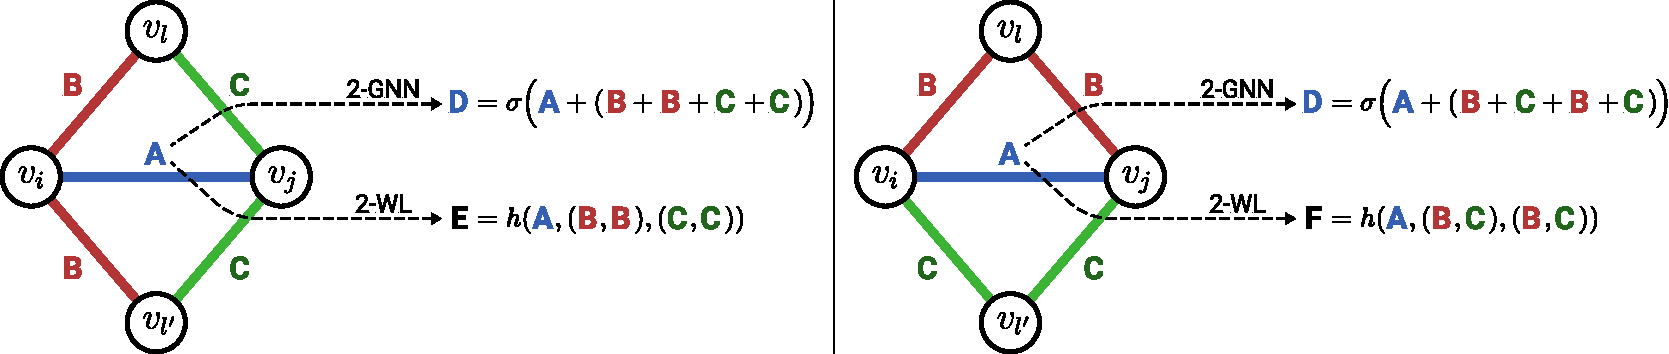
\includegraphics[width=\linewidth]{gfx/ltd/2gnn-2wl-diff.pdf}
	\caption[Edge colorings on which 2-\acsp{gnn} and 2-\acs{wl} behave differently.]{
		Two edge colorings on which 2-\acsp{gnn} and 2-\acs{wl} behave differently.
		A 2-\acs{gnn} will refine the ``color vector'' of $e_{ij}$ to \textsf{\textbf{\small\textcolor{t_blue}{D}}} for both initial colorings.
		2-\acs{wl} on the other hand differentiates both colorings by preserving the color tuple information.
	}\label{fig:ltd:2gnn-2wl-diff}
\end{figure}

We will now analyze what those different notions of neighborhood imply for the discriminative and computational power of 2-\acsp{gnn} in comparison to 2-\acs{wl}.
In the first step we show that the discriminative power of 2-\acsp{gnn} on all graphs $G \in \mathcal{G}$ is upper bounded by that of 1-\acs{wl} on the so-called \textit{edge neighborhood graphs} $G^{\mathcal{E}} \in \mathcal{G}^{\mathcal{E}}$.
\begin{defn}\label{defn:ltd:edge-graph}
	The \textit{edge neighborhood graph} of a given graph $G = (\mathcal{V}_G, \mathcal{E}_G)$ is defined as $G^{\mathcal{E}} \coloneqq (\mathcal{V}_{G^{\mathcal{E}}}, \mathcal{E}_{G^{\mathcal{E}}})$ with the vertices $\mathcal{V}_{G^{\mathcal{E}}} \coloneqq \{ \ldblbrace v, u \rdblbrace\, |\, (v, u) \in \mathcal{E}_G \lor v = u \}$ and the edges $\mathcal{E}_{G^{\mathcal{E}}} \coloneqq \left\{ (e, e') \in \mathcal{V}_{\mathcal{G}^{\mathcal{E}}}^2 |\, \left|e \cap e'\right| = 1 \right\}$. % chktex 21
\end{defn}
\begin{prop}\label{prop:ltd:2gnn-wl1-limit}
	The discriminative power of all 2-\acsp{gnn} $h_2$ is bounded by that of 1-\ac{wl} on edge neighborhood graphs, i.e.\ $\forall\, G, H \in \mathcal{G}: G^{\mathcal{E}} \mathrel{\simeq_1} H^{\mathcal{E}} \rightarrow h_2(G) = h_2(H)$. % chktex 21
\end{prop}
\begin{proof}
	By \cref{defn:ltd:edge-graph} it holds that $\forall e_{ij} \in \mathcal{E}_G: {\Gamma_G(v_i) \cup \Gamma_G(v_j)} = \Gamma_{G^{\mathcal{E}}}(e_{ij})$.
	Therefore the 2-\acs{gnn} convolution operation defined in \cfullref[ on ]{eq:related:kgnn-layer} can be rewritten as a vertex neighborhood convolution operator
	\begin{align*}
		Z_G^{(t)}[e] = \sigma\left( Z_G^{(t-1)}[e] W^{(t)} + \smashoperator[lr]{\sum_{e' \in \Gamma_{G^{\mathcal{E}}}(e)}} Z_G^{(t-1)}[e'] W_{\Gamma}^{(t)} \right)
		\text{.}
	\end{align*}
	\Cref{prop:ltd:2gnn-wl1-limit} then follows from \cref{prop:related:gcnn-wl1-limit}~(\cpageref{prop:related:gcnn-wl1-limit}).
\end{proof}
\begin{lem}\label{lem:ltd:wl1-regular-edge-neighbor-limit}
	1-\ac{wl} cannot distinguish the edge neighborhood graphs $G^{\mathcal{E}}$ and $H^{\mathcal{E}}$ of any pair of $d$-regular graphs $G$ and $H$ with $n$ vertices.
\end{lem}
\begin{proof}
	Let $G$ and $H$ be two $d$-regular graphs of size $n$.
	Their corresponding edge neighborhood graphs $G^{\mathcal{E}}$ and $H^{\mathcal{E}}$ both have $n^{\mathcal{E}} = n + \frac{nd}{2}$ vertices.
	$n$ of those edge neighborhood vertices correspond to the vertices of $G$ and $H$ respectively, we will refer to them as \textit{loop vertices} $L_G$/$L_H$.
	The remaining $\frac{nd}{2}$ edge neighborhood vertices correspond to the edges of $G$ and $H$, we will refer to them as \textit{edge vertices} $E_G$/$E_H$.

	W.l.o.g.\ we define the initial colors of the loop vertices as $\chi^{(0)}(v) = \textcolor{t_blue}{\texttt{A}}$ for all $v \in L_G \cup L_H$. % chktex 25
	The initial colors of the edge vertices are defined as $\chi^{(0)}(e) = \textcolor{t_red}{\texttt{B}}$ for all $e \in E_G \cup E_H$. % chktex 25
	Note that each loop vertex $\ldblbrace v_i, v_i \rdblbrace$ with $v_i \in \mathcal{V}_G \cup \mathcal{V}_H$ has $d$ neighbors, the edges incident to $v_i$.
	Similarly each edge vertex $\ldblbrace v_i, v_j \rdblbrace$ has $2d$ neighbors, two of which are the loop vertices $\ldblbrace v_i, v_i \rdblbrace$ and $\ldblbrace v_j, v_j \rdblbrace$ with the remaining $2d - 2$ neighbors corresponding to the edges that are incident to $e_{ij}$.
	This is illustrated in \cref{fig:ltd:edge-neighborhood}.

	After one color refinement step we get $\chi^{(1)}(v) = h(\textcolor{t_blue}{\texttt{A}}, \ldblbrace \underbrace{\textcolor{t_red}{\texttt{B}}, \dots, \textcolor{t_red}{\texttt{B}}}_{d\text{ times}} \rdblbrace) \eqqcolon \textcolor{t_blue}{\texttt{C}}$ for all loop vertices $v \in  L_G \cup L_H$ and $\chi^{(1)}(e) = h(\textcolor{t_red}{\texttt{B}}, \ldblbrace \textcolor{t_blue}{\texttt{A}}, \textcolor{t_blue}{\texttt{A}}, \underbrace{\textcolor{t_red}{\texttt{B}}, \dots, \textcolor{t_red}{\texttt{B}}}_{\mathclap{2d - 2 \text{ times}}} \rdblbrace) \eqqcolon \textcolor{t_red}{\texttt{D}}$. % chktex 25
	This means that $\chi^{(0)}$ and $\chi^{(1)}$ are identical up to the color substitutions $\textcolor{t_blue}{\texttt{A}} \to \textcolor{t_blue}{\texttt{C}}$ and $\textcolor{t_red}{\texttt{B}} \to \textcolor{t_red}{\texttt{D}}$, i.e.\ $\chi^{(0)} \equiv \chi^{(1)}$, which in turn implies that 1-\ac{wl} terminates after one iteration. % chktex 25
	\Cref{lem:ltd:wl1-regular-edge-neighbor-limit} then directly follows since both $G^{\mathcal{E}}$ and $H^{\mathcal{E}}$ have $n$ vertices with the final color $\textcolor{t_blue}{\texttt{C}}$ and $\frac{nd}{2}$ vertices with the final color $\textcolor{t_red}{\texttt{D}}$, i.e.\ $G^{\mathcal{E}} \mathrel{\simeq_1} H^{\mathcal{E}}$. % chktex 25
\end{proof}
\begin{figure}[ht]
	\centering
	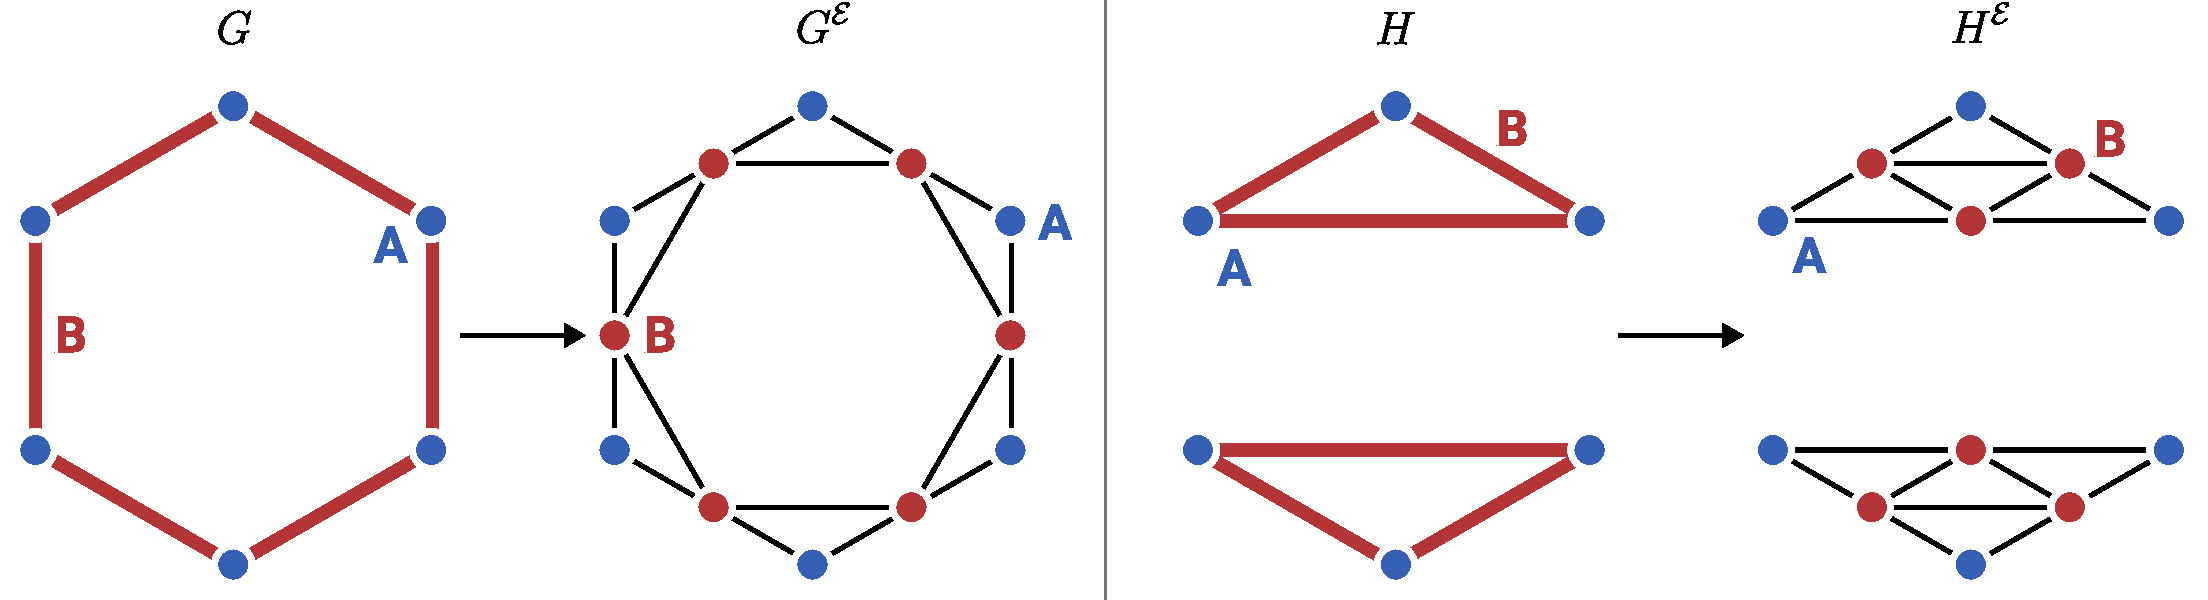
\includegraphics[width=\linewidth]{gfx/ltd/edge-neighborhood.pdf}
	\caption{
		Illustration of the edge neighborhood graphs of two 2-regular graphs of size 6.
	}\label{fig:ltd:edge-neighborhood}
\end{figure}
\begin{prop}\label{prop:ltd:2gnn-regular-limit}
	A 2-\acs{gnn} cannot distinguish regular graphs of the same size and therefore has a lower discriminative power than 2-\ac{wl}.
\end{prop}
\begin{proof}
	The proposition directly follows from \cref{prop:ltd:2gnn-wl1-limit}, \cref{lem:ltd:wl1-regular-edge-neighbor-limit} and the fact that 2-\acs{wl} is able to distinguish most regular graphs~\cite[cor.~1.8.6]{Immerman1990}.
\end{proof}

As described in \cref{sec:related:character:wl} the discriminative power of a model is, by itself, not necessarily relevant for real-world graph datasets.
In \cfullref[ on ]{prop:related:wl2-cycle-count} we saw however that 2-\acs{wl} not only has a higher discriminative power than 1-\acs{wl} but also that it is able to count the number of $m$-cycles in a given graph for all $m \leq 7$.
This is relevant because cycle counts are a commonly used metric in real-world domains such as social network and molecular structure analysis~\cite{Milo2002}\cite{Newman2003}\cite{Welser2007}\cite{Adamson1973}\cite{Kekule1866}.
To conclude this section we now show that 2-\acsp{gnn} not only have a lower discriminative power than 2-\acs{wl} but are also unable to detect cycles.
\begin{prop}
	2-\acsp{gnn} cannot detect $m$-cycles for all $m \geq 3$.
\end{prop}
\begin{proof}
	Let $n$ be the \ac{lcm} of $3$ and some $m > 3$.
	We define $c_3 \coloneqq \frac{n}{3}$ and $c_m \coloneqq \frac{n}{m}$.
	Based on that we define the following two graphs:
	Let $G_3$ be a graph consisting of $c_3$ disconnected cycles of length $3$, analogously let $G_m$ be a graph consisting of $c_m$ disconnected cycles of length $m$.
	Since both $G_3$ and $G_m$ are 2-regular and have the size $n$, any 2-\ac{gnn} $h_2: \mathcal{G} \to \mathcal{Y}$ must map both of them to the same $y \in \mathcal{Y}$ by \cref{prop:ltd:2gnn-regular-limit}.

	Let us assume that $h_2$ is able to detect cycles of length $3$, i.e.\ triangles.
	By \cfullref[ on ]{defn:related:wl-count-detect} this would imply that there is a function $g: \mathcal{Y} \to \{ 0, 1\}$ s.t.\ $g(h_2(G_3)) = g(y) = 1$ and $g(h_2(G_m)) = g(y) = 0\ \lightning$.
	Conversely, assuming that $h_2$ is able to detect cycles of length $m > 3$, we obtain the contradiction $g(h_2(G_3)) = g(y) = 0$  and $g(h_2(G_m)) = g(y) = 1\ \lightning$.
	This concludes the proof.
\end{proof}

In this section we compared 2-\acsp{gnn} with the 2-\acs{wl} algorithm and found that they have a significantly lower discriminative and computational power than 2-\acs{wl}.
Motivated by those limitations we describe a novel graph convolution operator which is closer to 2-\acs{wl} in the following section.

\section{A Novel 2-\acs*{wl} Inspired \acs*{gnn}}%
\label{sec:ltd:wl2gnn}

We have seen that the main difference between 2-\acsp{gnn} and 2-\acs{wl} is their notion of ``neighborhood''.
In this section we describe a novel convolution operator which uses edge tuple neighbors just like 2-\acs{wl} to overcome the limitations of 2-\acsp{gnn}.
This will be done in three steps:
\begin{enumerate*}
	\item We begin by formally defining the 2-\acs{wl} convolution operator.
	\item Then the discriminative and computational power of this operator are analyzed.
	\item Lastly we describe how 2-\acs{wl} convolutions can be implemented efficiently on a modern \ac{gpgpu}.
\end{enumerate*}

\subsection{Definition of the 2-\acs*{wl} Convolution Operator}%
\label{sec:ltd:wl2gnn:definition}

Similar to the 2-LWL kernel described in \cref{sec:related:gcr:kernel}, our 2-\acs{wl} convolution operator reduces the computational cost of 2-\acs{wl} via two simplifications:
\begin{enumerate}[label=\textbf{\arabic*.}]
	\item \textbf{2-multisets:}
		Since we assume that graphs are undirected, $e_{ij}$ and $e_{ji}$ have identical feature vectors $x[e_{ij}] = x[e_{ji}] \in \mathcal{X}_{\mathcal{E}}$ and the same 2-\acs{wl} neighborhood.
		Instead of refining/convolving the feature vectors of 2-tuples $(v_i, v_j)$ we can therefore refine/convolve the feature vectors of 2-multisets $\ldblbrace v_i, v_j \rdblbrace$.
		This halves the number of feature vectors without affecting the discriminative or computational power of the 2-\acs{wl} convolution operator.
		To simplify the notation we assume that $e_{ij} = e_{ji} = \ldblbrace v_i, v_j \rdblbrace$ in the rest of this section.
	\item \textbf{Neighborhood localization:}
		Using the 2-multiset simplification, the original 2-\acs{wl} algorithm refines the color of all multisets $e_{ij} \in \mathcal{V}_G^2$ by hashing its current color and the colors of all neighbors ${\{ \ldblbrace e_{il}, e_{lj} \rdblbrace \}}_{v_l \in \mathcal{V}_G}$.
		This means that the time complexity of a single refinement step is $\mathcal{O}(n^3)$ for $n \coloneqq \left| \mathcal{V}_G \right|$ which quickly becomes infeasible for large graphs.

		To address this issue we reduce both the number of colored edges as well as the number of neighbors of each edge.
		This is achieved by only considering the edges that are part of the so-called \textit{$r$-th power of a given graph $G$} where $r \in \mathbb{N}$ is the freely choosable \textit{neighborhood radius}.
		\begin{defn}
			The \textit{$r$-th power of a graph $G$} is defined as
			\begin{align*}
				G^r \coloneqq \left(\mathcal{V}_G, \left\{ e_{ij} \in \mathcal{V}_G^2\, |\, d_{\mathrm{SP}, G}(v_i, v_j) \leq r \right\}\right) % chktex 21
			\end{align*}
			where $d_{\mathrm{SP}, G}(v_i, v_j)$ is the length of the shortest path between $v_i$ and $v_j$ in $G$.
			The distance of a vertex $v_i \in \mathcal{V}_G$ to itself is defined as $d_{\mathrm{SP}, G}(v_i, v_i) \coloneqq 0$.
			Note that $G^1$ does not generally equal $G$ because $G^1$ has self-loop edges $e_{ii} \in \mathcal{E}_{G^1}$ at all vertices.
		\end{defn}
		For the neighborhood radius $r = 1$ only the self-loop edges ${\{ e_{ii} \}}_{v_i \in \mathcal{V}_G}$ and the edges $\mathcal{E}_{G}$ are considered;
		for $r > 1$ edges between indirectly connected vertices are considered as well.
		\Cref{fig:ltd:neighborhood-radius} illustrates this for varying neighborhood radii.
		Through the reduction of the considered edges, the neighbors of each $e_{ij} \in \mathcal{E}_{G^r}$ are in turn reduced to the common $r$-neighbors of $v_i$ and $v_j$, i.e.\ $\{ \ldblbrace e_{il}, e_{lj} \rdblbrace\, |\, v_l \in {\Gamma_{G^r}(v_i) \cap \Gamma_{G^r}(v_j)} \}$. % chktex 21
		\begin{figure}[t]
			\centering
			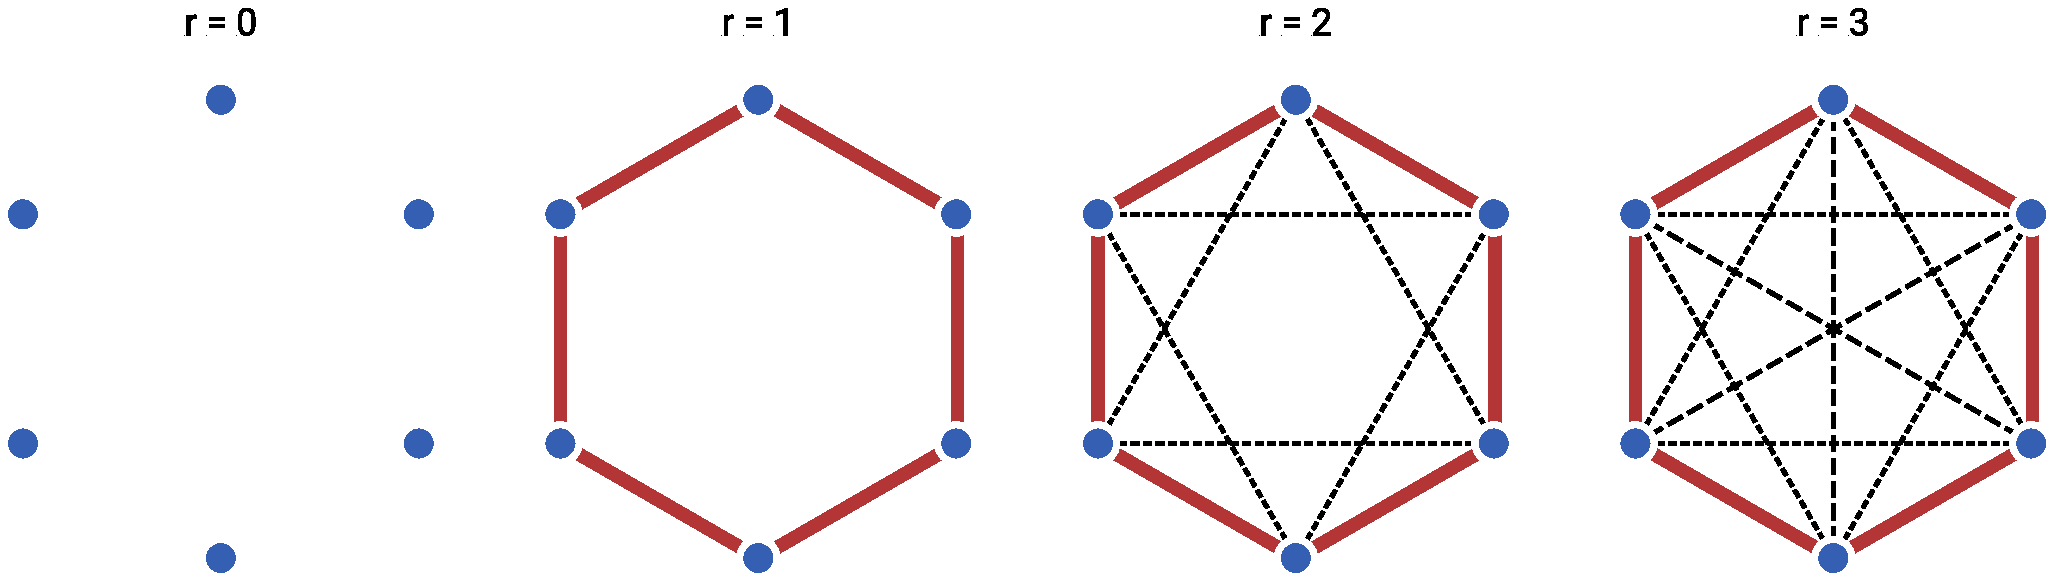
\includegraphics[width=0.9\linewidth]{gfx/ltd/neighborhood-radius.pdf}
			\caption[Illustration of the powers of the six-cycle graph.]{
				Illustration of the powers of the six-cycle graph for varying $r$.
				The self-loop edge at each of the vertices is not explicitly shown.
				For $r = 3$ all possible edges between the six vertices will be considered just as in the original 2-\acs{wl} algorithm.
			}\label{fig:ltd:neighborhood-radius}
		\end{figure}

		Let us now consider what the reduced number of considered edges and the reduced number of edge neighbors implies for the runtime of a refinement step.
		If $G$ is a sparse graph with the maximum vertex degree $d \coloneqq \max_{v \in \mathcal{V}_G} \left|\Gamma_G(v)\right|$, the number of considered edges is bounded by $\mathcal{O}(n d^r)$ where each edge has at most $\mathcal{O}(d^r)$ neighbors.
		Consequently the time complexity of a refinement step becomes $\mathcal{O}(n d^{2r})$ which is a significant improvement over the $\mathcal{O}(n^3)$ bound of a full 2-\acs{wl} refinement step (assuming $d \ll n$).
\end{enumerate}
Based on the 2-multiset and the neighborhood localization simplifications we can now define the 2-\ac{wl} convolution operator.
\begin{defn}\label{defn:ltd:wl2-conv-init}
	The \textit{initial feature matrix $Z_G^{(0)}$} of the 2-\acs{wl} convolution operator with the neighborhood radius $r \in \mathbb{N}$ contains both the vertex features $x[v_i] \in \mathcal{X}_{\mathcal{V}} = \mathbb{R}^{d_{\mathcal{V}}}$ as well as the edge features $x[e_{ij}] \in \mathcal{X}_{\mathcal{E}} = \mathbb{R}^{d_{\mathcal{E}}}$ of a given graph $G$.
	More specifically $Z_G^{(0)} \in \mathbb{R}^{{|\mathcal{E}_{G^r}|} \times (d_{\mathcal{V}} + d_{\mathcal{E}})}$ assigns a row vector $Z_G^{(0)}[e_{ij}]$ to all edges $e_{ij} \in \mathcal{E}_{G^r}$.
	Those initial edge feature vectors are defined by the following vector concatenation:
	\begin{align*}
		Z_G^{(0)}[e_{ij}] \coloneqq \left( \begin{cases}
			x[v_i] & \text{if $i = j$} \\
			\mathbf{0} & \text{else}
		\end{cases} \right) \oplus \left( \begin{cases}
			x[e_{ij}] & \text{if $e_{ij} \in \mathcal{E}_G$} \\
			\mathbf{0} & \text{else}
		\end{cases} \right)
	\end{align*}
\end{defn}
\begin{defn}\label{defn:ltd:wl2-conv-step}
	We define the \textit{2-\acs{wl} graph convolution operator} as
	\begin{gather*}
		Z_G^{(t)}[e_{ij}] \coloneqq \sigma\left( Z_G^{(t-1)}[e_{ij}] W_{\mathrm{L}}^{(t)} + \smashoperator[lr]{\sum_{v_l \in {\Gamma_{G^r}(v_i) \cap \Gamma_{G^r}(v_j)}}} \kappa^{(t)}\left( Z_G^{(t-1)}[e_{ij}], \ldblbrace Z_G^{(t-1)}[e_{il}], Z_G^{(t-1)}[e_{lj}] \rdblbrace \right) \right) \\
		\text{with } \kappa^{(t)}(z_{ij}, \ldblbrace z_{il}, z_{lj} \rdblbrace) \coloneqq \left( z_{ij} W_{\mathrm{F}}^{(t)} \right) \odot \sigma_{\Gamma}\left(\left( z_{il} + z_{lj} \right) W_{\Gamma}^{(t)} \right)
		\text{.}
	\end{gather*}
\end{defn}
The convolution operator from \cref{defn:ltd:wl2-conv-step} is parameterized by the three matrices $W_{\mathrm{L}}^{(t)}, W_{\mathrm{F}}^{(t)},  W_{\Gamma}^{(t)} \in \mathbb{R}^{d^{(t-1)} \times d^{(t)}}$ and uses two freely choosable activation functions $\sigma$ and $\sigma_{\Gamma}$.
There are three properties which motivate this particular choice of convolution layer:
\begin{enumerate}[label=\textbf{\arabic*.}]
	\item \textbf{Simulation of \acp{mlp}:}
		By choosing $W_{\mathrm{F}}^{(t)} = \mathbf{0}$ the convolution behaves like a regular fully connected layer.
		A stack of 2-\acs{wl} convolution layers can therefore simulate arbitrary \acp{mlp}.
	\item \textbf{Perservation of edge pair information:}
		The 2-\acs{wl} convolution layer computes a feature vector for each neighbor $\ldblbrace e_{il}, e_{lj} \rdblbrace$ of $e_{ij}$ via $\sigma_{\Gamma}\left(\left( z_{il} + z_{lj} \right) W_{\Gamma}^{(t)} \right)$.
		A 2-\acs{gnn} use a similar formulation but leaves out the inner nonlinearity $\sigma_{\Gamma}$;
		as we saw in \cref{fig:ltd:2gnn-2wl-diff} this causes 2-\acsp{gnn} to lose the edge pair information due to the commutativity and associativity of $+$.
	\item \textbf{Context-dependent neighborhood filtering:}
		Instead of filtering out all neighbors, $W_{\mathrm{F}}^{(t)}$ also allows to filter the neighborhood of $e_{ij}$ more selectively.
		We can interpret $z_{ij} W_{\mathrm{F}}^{(t)} \in \mathbb{R}^{d^{(t)}}$ as a row vector of feature dimension weights.
		The feature dimensions of neighbors are rescaled via those weights which allows the model to aggregate different types of neighbors depending on $z_{ij}$.
\end{enumerate}

\subsection{Expressive Power of 2-\acs*{wl}-\acsp*{gnn}}%
\label{sec:ltd:wl2gnn:properties}

In this section we will analyze the discriminative and computational power of the 2-\ac{wl} convolution operator that was just defined.
We begin by showing that 2-\acs{wl}-\acsp{gnn} are at least as powerful as 1-\acs{wl}.

\begin{defn}\label{defn:ltd:vert-conv}
	A \ac{gnn} $h_1: \mathcal{G} \to \mathcal{Y}$ uses \textit{weighted vertex neighborhood sums} if its convolutional layers can be described by
	\begin{align*}
		Z_{G}^{(t)}[v_i] = \mathrm{\acs*{mlp}}^{(t)}\left( w_{ii} Z_{G}^{(t-1)}[v_i] + \smashoperator[lr]{\sum_{v_j \in \Gamma_G(v_i)}} w_{ij} Z_{G}^{(t-1)}[v_l] \right)
		\text{.}
	\end{align*}
\end{defn}
\Cref{defn:ltd:vert-conv} includes \acp{gcn}~\cite{Kipf2017} where the \ac{mlp} only consists of a single layer and the weights are $w_{ij} = {\left(\left| \Gamma_G(v_i) \right| + 1\right)}^{-\frac{1}{2}}{\left(\left| \Gamma_G(v_j) \right| + 1\right)}^{-\frac{1}{2}}$ (see \cfullref{eq:related:gcn-wl1}).
\Acp{gin}~\cite{Xu2018} also trivially satisfy the definition (see \cfullref{eq:related:gin-layer}).
\begin{thm}\label{thm:ltd:wl2-simulation}
	For each \ac{gnn} $h_1$ that uses weighted vertex neighborhood sums, there is a 2-\acs{wl}-\acs{gnn} $h_2$ which simulates $h_1$, i.e.\ $\forall G \in \mathcal{G}: h_1(G) = h_2(G)$.
\end{thm}
\begin{proof}
	We prove the theorem by construction.
	Let $G \in \mathcal{G}$ be an arbitrary input graph with $n \coloneqq \left|\mathcal{V}_G\right|$ and $m \coloneqq n + \left|\mathcal{E}_G\right|$.
	By definition $h_1$ is a \ac{gnn} of the form $\mathit{Pool}_1(\mathit{Conv}_1(G))$ where $\mathit{Conv}_1$ is a stack of $T$ weighted vertex neighborhood sum convolutions ${\left\{ S^{(t)}: \mathbb{R}^{n \times d^{(t-1)}} \to \mathbb{R}^{n \times d^{(t)}} \right\}}_{t=1}^T$ with each corresponding $\mathrm{\acs*{mlp}}^{(t)}$ having $K$ layers. % chktex 21
	$\mathit{Pool}_1$ combines the vertex feature vectors produced by $\mathit{Conv}_1$.

	Let $h_2$ be a \ac{gnn} of the form $\mathit{Pool}_2(\mathit{Conv}_2(G))$ where $\mathit{Conv}_2$ is a stack of $(2 + K) T$ 2-\acs{wl} convolution layers ${\left\{ S^{(t, k)}: \mathbb{R}^{m \times d^{(t,k-1)}} \to \mathbb{R}^{m \times d^{(t,k)}} \right\}}_{(t, k) \in [T] \times [2+K]}$ with the neighborhood radius $r \coloneqq 1$. % chktex 21
	Thus $\mathit{Conv}_2$ produces a feature vector for each of the $m$ edges of $G^1$, i.e.\ one for each vertex and each edge of $G$.
	We denote the initial 2-\acs{wl} feature matrix with $Z^{(1,0)} \in \mathbb{R}^{m \times d^{(0,0)}}$.
	The layers ${\left\{ S^{(t, 2 + K)} \right\}}_{t=1}^T$ produce the feature matrices $Z^{(t, 2 + K)} = Z^{(t + 1, 0)}$ which are then fed as input into the successor layer $S^{(t + 1, 1)}$. % chktex 21
	Intuitively $\mathit{Conv}_2$ simulates each layer of $\mathit{Conv}_1$ via a stack of $2 + K$ 2-\acs{wl} convolution layers.
	This is illustrated in \cref{fig:ltd:wl2-simulation}.
	\begin{figure}[ht]
		\centering
		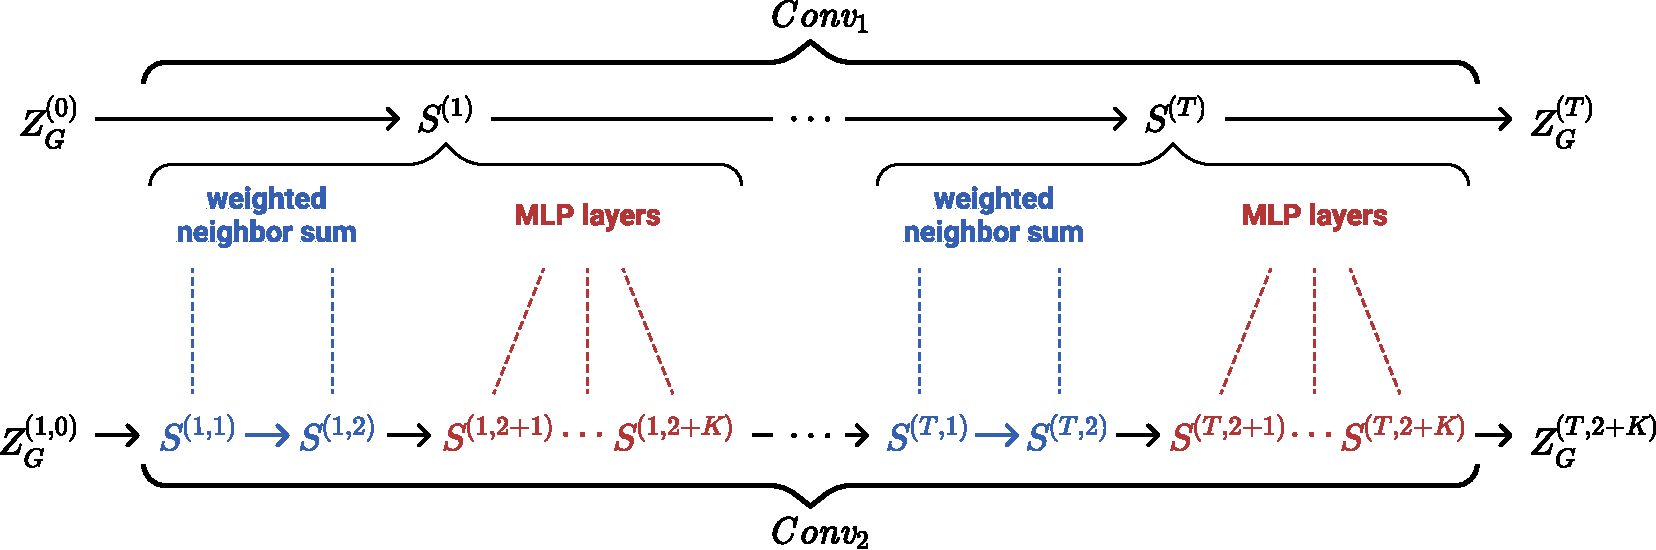
\includegraphics[width=\linewidth]{gfx/ltd/wl2-simulation.pdf}
		\caption[Illustration of a 2-\acs{wl}-\acs{gnn} architecture that simulates vertex neighborhood convolutions.]{
			Illustration of the correspondence between $\mathit{Conv}_1$ and $\mathit{Conv}_2$.
		}\label{fig:ltd:wl2-simulation}
	\end{figure}

	Let $\varphi: \mathbb{R}^{d^{(T, 2 + K)}} \to \mathbb{R}^{d^{(T)}} \cup \{ \texttt{nil} \}$ be a function which maps the final 2-\acs{wl} feature vectors produced by $\mathit{Conv}_2$ to the output space of $\mathit{Conv}_1$ or the constant \texttt{nil}.
	Let $\mathit{Pool}_2\left(Z_G^{(T,2+K)}\right) \coloneqq \mathit{Pool}_1(\ldblbrace z_{ij}\, |\, z_{ij} = \varphi\left(Z_G^{(T,2+K)}[e_{ij}]\right) \land e_{ij} \in \mathcal{E}_{G^1} \land z_{ij} \neq \texttt{nil} \rdblbrace)$.
	\Cref{thm:ltd:wl2-simulation} then follows if there is a function $\varphi$ s.t.\ $\forall v_i \in \mathcal{V}_G: \mathit{Conv}_1(G)[v_i] = \varphi(\mathit{Conv}_2(G)[e_{ii}])$ and $\forall e_{ij} \in \mathcal{E}_G: \varphi(\mathit{Conv}_2(G)[e_{ij}]) = \texttt{nil}$.
	To guarantee that there is such a function $\varphi$ we now inductively prove the following three invariants which have to hold for all $t \in \{ 0, \dots, T \}$:
	\begin{enumerate}[label={(P\arabic*)}]
		\item\label{inv:ltd:wl2-simulation:indicator}
			${Z_G^{(t,2+K)}[e_{ij}]}_1 = \mathbbm{1}[i = j]$, i.e.\ the first component of each 2-\acs{wl} feature vector allows $\varphi$ to decide whether that vector should be mapped to \texttt{nil}.
		\item\label{inv:ltd:wl2-simulation:feature}
			${Z_G^{(t,2+K)}[e_{ii}]}_{2, \dots, (d^{(t)} + 1)} = Z_G^{(t)}[v_{i}]$, i.e.\ the second to $(1 + d^{(t)})$-th components of each self-loop feature vector in $h_2$ contain the corresponding convolved vertex feature vector at layer $t$ in $h_1$.
		\item\label{inv:ltd:wl2-simulation:weight}
			${Z_G^{(t,2+K)}[e_{ij}]}_{d^{(t)} + 2} = w_{ij}$, i.e.\ the weights for the vertex neighborhood sums are encoded in the edge and self-loop feature vectors.
	\end{enumerate}
	For $t = 0$ all three invariants hold by \cref{defn:ltd:wl2-conv-init}:
	\begin{align*}
		\forall v_i \in \mathcal{V}_G: Z_G^{(1, 0)}[e_{ii}] \coloneqq (1) \oplus x[v_i] \oplus (w_{ii})
		\text{ and }
		\forall e_{ij} \in \mathcal{E}_G: Z_G^{(1, 0)}[e_{ij}] \coloneqq (0) \oplus \mathbf{0} \oplus (w_{ij})
		\text{.}
	\end{align*}
	Assuming the invariants hold for $t - 1$ we now show that they also hold for $t$.
	As illustrated in \cref{fig:ltd:wl2-simulation} the layers $S^{(t, 1)}$ and $S^{(t, 2)}$ should compute the weighted vertex neighborhood sums
	\begin{align*}
		{Z^{(t, 2)}[e_{ii}]}_{2, \dots, (1+d^{(t-1)})} = w_{ii} {Z^{(t, 0)}[e_{ii}]}_{2, \dots, (1+d^{(t-1)})} + \smashoperator[lr]{\sum_{v_j \in \Gamma_G(v_i)}} w_{ij} {Z^{(t, 0)}[e_{jj}]}_{2, \dots, (1+d^{(t-1)})}
		\text{.}
	\end{align*}
	We now explicitly define parameter matrices for $S^{(t, 1)}$ and $S^{(t, 2)}$ s.t.\ this weighted sum is produced.
	Note that the weighted vertex neighborhood sum only requires scalar multiplication and vector addition, i.e.\ the $d^{(t-1)}$ vertex feature dimensions are mutually independent.
	W.l.o.g.\ this allows us to simplify notation by treating the vertex feature vectors as if they were scalars in the following definitions, i.e.\ we can assume $d^{(t-1)} = 1$ and $Z^{(t,0)}[e_{ii}] = (1, Z^{(t-1)}[v_i], w_{ii}) \in \mathbb{R}^{3}$.
	The layer $S^{(t, 1)}$ is defined by
	\begin{gather*}
		\begin{aligned}
			Z^{(t,1)}[e_{ij}] &= \textcolor{t_blue}{Z^{(t,0)}[e_{ij}] W_{\mathrm{L}}^{(t,1)}} + \smashoperator[lr]{\sum_{v_l \in {\Gamma_{G^1}(v_i) \cap \Gamma_{G^1}(v_j)}}} \textcolor{t_red}{\left( Z^{(t,0)}[e_{ij}] W_{\mathrm{F}}^{(t,1)}\right)} \odot \textcolor{t_darkgreen}{\left( \left( Z^{(t,0)}[e_{il}] + Z^{(t,0)}[e_{lj}] \right) W_{\Gamma}^{(t,1)} \right)} \\ % chktex 25
			&= \begin{cases}
				\textcolor{t_blue}{(1, 0, w_{ii}, 0)} + \textcolor{t_darkgreen}{\left(0, 0, 0, 2\textcolor{t_red}{w_{ii}} Z^{(t-1)}[v_i]\right)} + \smashoperator[lr]{\sum_{v_l \in \Gamma_{G^1}(v_i)}} \textcolor{t_darkgreen}{\left(0, w_{il} \textcolor{t_red}{Z^{(t-1)}[v_i]}, 0, 0\right)} & \text{if $i = j$} \\ % chktex 25
				\textcolor{t_blue}{(0, 0, w_{ij}, 0)} + \textcolor{t_darkgreen}{\left(0, 0, 0, \textcolor{t_red}{w_{ij}} Z^{(t-1)}[v_i]\right)} + \textcolor{t_darkgreen}{\left(0, 0, 0, \textcolor{t_red}{w_{ij}} Z^{(t-1)}[v_j]\right)} & \text{else} % chktex 25
			\end{cases} \\
			&= \begin{cases}
				\left(1, \mkern6mu\smashoperator[lr]{\sum_{v_l \in \Gamma_{G^1}(v_i)}} w_{il} Z^{(t-1)}[v_i], w_{ii}, 2 w_{ii} Z^{(t-1)}[v_i] \right) & \text{if $i = j$} \\
				\left(0, 0, w_{ij}, w_{ij} (Z^{(t-1)}[v_i] + Z^{(t-1)}[v_j])\right) & \text{else}
			\end{cases}
		\end{aligned}\\
		\text{with }
		W_{\mathrm{L}}^{(t,1)} \coloneqq \begin{pmatrix}
			\textcolor{t_blue}{1} & 0 & 0 & 0 \\ % chktex 25
			0 & 0 & 0 & 0 \\
			0 & 0 & \textcolor{t_blue}{1} & 0 % chktex 25
		\end{pmatrix},
		W_{\mathrm{F}}^{(t,1)} \coloneqq \begin{pmatrix}
			0 & 0 & 0 & 0 \\
			0 & \textcolor{t_red}{\frac{1}{2}} & 0 & 0 \\ % chktex 25
			0 & 0 & 0 & \textcolor{t_red}{1} % chktex 25
		\end{pmatrix},
		W_{\Gamma}^{(t,1)} \coloneqq \begin{pmatrix}
			0 & 0 & 0 & 0 \\
			0 & 0 & 0 & \textcolor{t_darkgreen}{1} \\ % chktex 25
			0 & \textcolor{t_darkgreen}{1} & 0 & 0 % chktex 25
		\end{pmatrix}
		\text{.}
	\end{gather*}
	The vertex neighborhood summation is completed via $S^{(t, 2)}$ which is defined by
	\begin{gather*}
		\begin{aligned}
			Z^{(t,2)}[e_{ij}] &= \begin{cases}
				\textcolor{t_blue}{\left(1, -\smashoperator[lr]{\sum_{v_l \in \Gamma_{G^1}(v_i)}} w_{il} Z^{(t-1)}[v_i], w_{ii} \right)} + \smashoperator[lr]{\sum_{v_l \in \Gamma_{G^1}(v_i)}} \textcolor{t_darkgreen}{\left(0, w_{il}\left(Z^{(t-1)}[v_i] + Z^{(t-1)}[v_l]\right), 0\right)} & \text{if $i = j$} \\ % chktex 25
				\textcolor{t_blue}{(0, 0, w_{ij})} & \text{else} % chktex 25
			\end{cases} \\
			&= \begin{cases}
				\left(1, w_{ii} Z^{(t-1)}[v_i] + \smashoperator[lr]{\sum_{v_l \in \Gamma_{G}(v_i)}} w_{il} Z^{(t-1)}[v_l], w_{ii}\right) & \text{if $i = j$} \\
				(0, 0, w_{ij}) & \text{else}
			\end{cases}
		\end{aligned}\\
		\text{with }
		W_{\mathrm{L}}^{(t,2)} \coloneqq \begin{pmatrix}
			\textcolor{t_blue}{1} & 0 & 0 \\ % chktex 25
			0 & \textcolor{t_blue}{-1} & 0 \\ % chktex 25
			0 & 0 & \textcolor{t_blue}{1} \\ % chktex 25
			0 & 0 & 0
		\end{pmatrix},\quad
		W_{\mathrm{F}}^{(t,2)} \coloneqq \begin{pmatrix}
			0 & \textcolor{t_red}{\frac{1}{2}} & 0 \\ % chktex 25
			0 & 0 & 0 \\
			0 & 0 & 0 \\
			0 & 0 & 0
		\end{pmatrix},\quad
		W_{\Gamma}^{(t,2)} \coloneqq \begin{pmatrix}
			0 & 0 & 0 \\
			0 & 0 & 0 \\
			0 & 0 & 0 \\
			0 & \textcolor{t_darkgreen}{1} & 0 % chktex 25
		\end{pmatrix}
		\text{.}
	\end{gather*}
	Using the two layers $S^{(t, 1)}$ and $S^{(t, 2)}$ that we just defined, the weighted vertex neighborhood sum for all $v_i \in \mathcal{V}_G$ is contained in $Z^{(t,2)}[e_{ii}]$.
	Additionally for all $e_{ij} \in \mathcal{E}_{G^1}$ the indicators ${Z^{(t,2)}[e_{ij}]}_1 = \mathbbm{1}[i = j]$ and the weights ${Z^{(t,2)}[e_{ij}]}_{d^{(t)} + 2} = w_{ij}$ are preserved.
	This means that the invariants~\ref{inv:ltd:wl2-simulation:indicator} and~\ref{inv:ltd:wl2-simulation:weight} are satisfied after $S^{(t, 2)}$.
	To complete the induction step it now remains to show that all three invariants hold after applying the layers $S^{(t, 2+1)}, \dots, S^{(t, 2+K)}$.
	As previously mentioned, a 2-\acs{wl} convolution layer is reduced to a fully connected layer if $W_{\mathrm{F}}^{(t)} = \mathbf{0}$.
	Via the universal approximation theorem~\cite{Hornik1991} we can therefore use $S^{(t, 2+1)}, \dots, S^{(t, 2+K)}$ to simulate the $K$ layers of $\mathrm{\acs*{mlp}}^{(t)}$ without changing the first and last dimension of each feature vector to preserve the invariants~\ref{inv:ltd:wl2-simulation:indicator} and~\ref{inv:ltd:wl2-simulation:weight}.
	The resulting feature matrix $Z^{(t,2+K)}$ then satisfies all three invariants which completes the induction.

	Using invariants~\ref{inv:ltd:wl2-simulation:indicator} and~\ref{inv:ltd:wl2-simulation:feature} for $t = T$ we can therefore set
	\begin{align*}
		\varphi\left(Z_G^{(T,2+K)}[e_{ij}]\right) \coloneqq \begin{cases}
			{Z_G^{(T,2+K)}[e_{ij}]}_{2, \dots, (d^{T} + 1)} & \text{if ${Z_G^{(T,2+K)}[e_{ij}]}_1 = 1$} \\
			\texttt{nil} & \text{else}
		\end{cases}
		\text{.}
	\end{align*}
	By our previous definition of $\mathit{Pool}_2$, this in turn implies that $\mathit{Pool}_2(Z_G^{(T,2+K)}) = \mathit{Pool}_1(Z_G^{(T)}) \iff h_2(G) = h_1(G)$ which concludes the proof.
\end{proof}
\begin{cor}\label{cor:ltd:wl2-gnn-wl1-power}
	2-\acs{wl}-\acsp{gnn} have at least the same discriminative power as 1-\acs{wl}.
\end{cor}
\begin{proof}
	The corollary directly follows from the fact that 2-\acs{wl}-\acsp{gnn} can simulate \acp{gin} by \cref{thm:ltd:wl2-simulation} and the fact that \acp{gin} have the same discriminative power as 1-\acs{wl} by \cref{prop:related:gcnn-wl1-limit} (see \cpageref{prop:related:gcnn-wl1-limit}) because they use injective vertex neighborhood hashing functions~\cite{Xu2018}.
\end{proof}

To complete our analysis of the expressive power of 2-\acs{wl}-\acsp{gnn} we now show that they are not just as powerful as 1-\acs{wl} but in fact more powerful than 1-\acs{wl}.
\begin{prop}\label{cor:ltd:wl2-gnn-regular}
	There are $d$-regular graphs $G$ and $H$ of size $n$ which can be distinguished by 2-\acs{wl}-\acsp{gnn}.
\end{prop}
\begin{proof}
	The proposition follows if we choose the six-cycle graph for $G$ and the two three-cycles graph for $H$, both of which should be well-known at this point.
	Let $h_2 = \mathit{Pool} \circ S$ be a 2-\acs{wl}-\acs{gnn} with the neighborhood radius $r = 1$ which consists of a single 2-\acs{wl} convolution layer $S: \mathbb{R}^{* \times 2} \to \mathbb{R}^{* \times 1}$ and the pooling layer $\mathit{Pool} = \min$.
	In accordance with \cref{defn:ltd:wl2-conv-init} we set the initial feature vectors of the vertices $v_i$ of $G$ and $H$ to $Z^{(0)}[e_{ii}] \coloneqq (1, 0)$ and the initial feature vectors of their edges $e_{ij}$ to $Z^{(0)}[e_{ij}] \coloneqq (0, 1)$.
	Let the weight matrices of $S$ be $W_{\mathrm{L}} \coloneqq \mathbf{0}$ and $W_{\mathrm{F}} = W_{\Gamma} \coloneqq \begin{pmatrix} 1\\1 \end{pmatrix}$.
	For simplicity we choose the identity activation functions $\sigma = \sigma_{\Gamma} = \mathrm{id}$.

	By \cref{defn:ltd:wl2-conv-step} all self-loops $e_{ii}$ of $G^1$ and $H^1$ have the three neighbors $\{ \textcolor{t_blue}{\ldblbrace e_{ii}, e_{ii} \rdblbrace},\allowbreak \textcolor{t_red}{\ldblbrace e_{ij}, e_{ji} \rdblbrace},\allowbreak \textcolor{t_darkgreen}{\ldblbrace e_{il}, e_{li} \rdblbrace} \}$, i.e.\ the length-two walk along $e_{ii}$ itself and the length-two walks to and from the two neighboring vertices $\Gamma(v_i) = \{ v_j, v_l \}$. % chktex 25
	Therefore the convolved feature vector of all self-loops are $Z^{(1)}[e_{ii}] = (1) \odot (\textcolor{t_blue}{(1 + 1)} + \textcolor{t_red}{(1 + 1)} + \textcolor{t_darkgreen}{(1 + 1)}) = 6$. % chktex 25
	However for the non-self-loops of $G^1$ and $H^1$, i.e.\ the edges of $G$ and $H$, we get differing convolved feature vectors.
	The 2-\acs{wl} neighbors of $e_{ij} \in \mathcal{E}_G$ are $\{ \ldblbrace e_{ii},  e_{ij} \rdblbrace,\allowbreak \ldblbrace e_{ij}, e_{jj} \rdblbrace \}$.
	The 2-\acs{wl} neighbors of $e_{ij}' \in \mathcal{E}_H$ are $\{ \ldblbrace e_{ii}',  e_{ij}' \rdblbrace,\allowbreak \ldblbrace e_{ij}',  e_{jj}' \rdblbrace,\allowbreak \ldblbrace e_{il}',  e_{lj}' \rdblbrace \}$ where $v_l' \in \mathcal{V}_H$ is the common neighbor of $v_i'$ and $v_j'$.
	The different neighborhood sizes of the edges of $G$ and $H$ imply that $\forall e_{ij} \in \mathcal{E}_G: Z^{(1)}[e_{ij}] = 4$ while $\forall e_{ij}' \in \mathcal{E}_H: Z^{(1)}[e_{ij}] = 6$.
	Thus $h_2(G) = \min\{ 4, 6 \} \neq \min\{ 6, 6 \} = h_2(H)$ which concludes the proof. % chktex 21
\end{proof}
\begin{cor}\label{cor:ltd:wl2-gnn-more-wl1-power}
	The discriminative power of 2-\acs{wl}-\acsp{gnn} is strictly greater than that of the 1-\acs{wl} algorithm.
\end{cor}
\begin{proof}
	The corollary directly follows from \cref{cor:ltd:wl2-gnn-wl1-power} and \cref{cor:ltd:wl2-gnn-regular} since 1-\acs{wl} cannot distinguish regular graphs~\cite[cor.~1.8.5]{Immerman1990}.
\end{proof}

This concludes our analysis of the expressive power of 2-\acs{wl}-\acsp{gnn}.
The key takeaway from this section is that 2-\acs{wl}-\acsp{gnn} are more powerful than all vertex neighborhood aggregation \acp{gcnn} because the power of the latter is upper bounded by 1-\acs{wl}.
Additionally we can conclude that 2-\acs{wl}-\acsp{gnn} are in fact also more powerful than 2-\acsp{gnn} due to \cref{prop:ltd:2gnn-regular-limit}.
A more thorough discussion of the relation between 2-\acs{wl}-\acsp{gnn} and 2-\acs{wl} is left for future work.

\subsection{Implementation of 2-\acs*{wl}-\acsp*{gnn} on \acsp*{gpgpu}}%
\label{sec:ltd:wl2gnn:implementation}
